Neste capítulo, é detalhado o framework proposto para análise
preditiva das tendências das eleições presidenciais no Brasil
com base na análise de sentimentos dos dados do Twitter.
Conforme mostrado na Figura \ref{diagrama}, o framework é dividido em
cinco blocos, que são descritos nas subseções de \ref{extract} a \ref{sec:am}.


\figuraBib{diagrama}{ Diagrama em blocos do framework proposto para análise preditiva espaço-temporal com base nos dados do Twitter}{}{diagrama}{width=0.9\textwidth}%


\section{Extração de Dados}
\label{extract}

O primeiro bloco da Figura \ref{diagrama} corresponde ao rastreamento
e extração de \textit{tweets}. Neste bloco, os tweets são extraídos do
banco de dados do \textit{Twiter} disponível na Internet. Como a nova
versão da \acrshort{API} dessa rede social não permite extrair tweets para datas
anteriores a uma semana, foi necessário desenvolver um \textit{Web Crawler}, ou seja, um aplicativo usando a linguagem \textit{Python}
com a biblioteca \textit{Scrapy}. As datas usadas para a extração de
tweets foram uma semana antes do primeiro dia da eleição e no
próprio dia da eleição. Este procedimento foi replicado para
o segundo turno das eleições. Os dados utilizados neste trabalho são referentes às eleições de 2014, onde o segundo turno
foi disputado entre os candidatos Aécio Neves e Dilma Rousseff.


Todos os tweets foram coletados em um intervalo pré-definido
como o argumento do mecanismo de busca de tweets.
Como é necessário aplicar as técnicas de Processamento de
Linguagem Natural (PLN) em português, a preferência foi
dada aos conteúdos escritos naquela língua. Foram utilizados mais de 100.000 tweets para desenvolver o modelo de aprendizado de máquina e quatro algoritmos de classificação foram considerados para a validação do modelo.


Além do texto do \textit{tweet}, algumas outras informações coletadas
incluem autor, data, contagem de retweets, contagem de
favoritos, localização, menções, hashtags, ID de publicação e
link de publicação. Essas informações são organizadas em uma estrutura de dados denominada \textit{dataframe}, que é semelhante a uma matriz, mas contém o nome de cada 
coluna.


Para manipular os dados em formato de \textit{dataframe}, foi utilizada a biblioteca \textit{Pandas},
que facilita todo o processo de manipulação de dados ~\cite{mckinney2011pandas}. Na Figura \ref{dataframe} apresenta um exemplo de dataframe contendo os dados utilizados para realizar a análise.

\figuraBib{dataframe}{Dataframe com os dados utilizados para realizar as análises}{}{dataframe}{width=0.9\textwidth}%


\section{Pré-processamento de dados}
\label{sec:limpeza}

O segundo bloco da Figura \ref{diagrama} corresponde ao pré-processamento
de dados. As redes sociais apresentam múltiplos
públicos e a intensidade da emoção é o fator que diferencia um tweet de outro, onde intensidade se refere ao
grau ou quantidade de uma emoção, como positivo, negativo ou neutro.
Uma estratégia usual é considerar que todas as mensagens
coletadas têm a mesma importância ~\cite{de2015estrategia}.
Não há padrão de escrita definido para ser usado em redes
sociais. Consequentemente, foi necessário realizar a limpeza
de dados para padronizar as sentenças. Além disso, como estamos analisando um processo sério, que são as eleições presidenciais, todos os emoticons foram desconsiderados. O fluxo de limpeza de dados pode
ser visto na Figura ~\ref{limpeza}.


 \figuraBib{limpeza}{Fluxo de pré-processamento de dados}{}{limpeza}{width=0.8\textwidth}%


Foram definidas seis etapas para a limpeza dos dados, conforme pode ser visualizado na Figura ~\ref{limpeza}. 
A primeira etapa é responsável por remover tags de retweet e menções de profile. 
A segunda e terceira etapas tratam da remoção de links de sites e de acentos e pontuações, respectivamente.
 Em seguida, todas as stopwords em português e os espaços desnecessários são removidos na quarta e quinta etapas, respectivamente. 
 Por fim, a sexta etapa trata da conversão dos tweets para letras minúsculas.


As \textit{Stop Words} são freqüentemente usadas em sentenças
que desempenham um papel muito pequeno na análise de sentimento e, consequentemente, devem ser removidas ~\cite{sharma}.
Eles não contribuem para o processo de análise de sentimento
e apenas retardam o processo. Além disso, os dados devem ser
submetidos a um processo de stemming em que as palavras
são reduzidas ao seu radical ~\cite{de2015estrategia}.

    Na Tabela \ref{tb:limpeza}, mostra um exemplo de a limpeza de um tweet selecionado aleatoriamente do \textit{dataframe} utilizado para análise.


\begin{table}
    \centering
    \caption{Exemplo de limpeza de textos extraídos do \textit{Twitter}}
    \label{tb:limpeza}
    
    \begin{tabular}{l|p{8cm}} 
    \hline
    Etapa Inicial       & Mais uma vez @AecioNeves perde em Minas.   Não seria a hora de ele se desculpar com o estado,   ao invés de continuar.  \#Eleições https:/bit.ly/twitter \\ \hline
    1) Remoção de Hashtags  e Menções a Perfis  & Mais uma vez    perde em Minas. Não seria a hora de ele se desculpar com o estado, ao invés de continuar. https:/bit.ly/twitter \\ \hline
    2) Remoção de Links                                                                  & Mais uma      vez perde em Minas. Não seria a hora de ele se desculpar com o estado, ao invés de continuar.   \\ \hline                                                                                                                                                    
    3) Remoção de Pontuação e  Acentuação                                               & Mais uma      vez perde em Minas Nao seria a hora de ele se desculpar com o estado ao inves de continuar  \\ \hline                                                                                                                                             
    4) Remoção de Stopwords                                                              & perde em Minas  seria  hora  desculpar  estado  inves continuar \\ \hline                                                                                                                                                                                         
    5) Remoção de Espaços Desnecessários                                             & perde em Minas seria hora desculpar estado invés continuar   \\ \hline                                                                                                                                                                                            
    6) Converter para minúsculo                                                          & perde em minas seria hora desculpar estado invés continuar  \\ \hline                                                                                                                                                                                                   
    \end{tabular}
    \end{table}



No apêndice \ref{cod:limpeza}   o código utilizado para a limpeza e estruturação dos dados é apresentado Foram utilizadas 
expressões regulares para substituir carácteres especiais, possibilitando a aplicação do processo de stemming numa etapa 
posterior.



\section{Análise de Sentimentos}

O terceiro bloco da Figura \ref{diagrama} corresponde à análise de sentimentos. 
Neste trabalho foram utilizadas as bibliotecas TextBlob} e OpLexicon para processamento de texto. A Tabela \ref{table1} mostra as
porcentagens de polaridade para cada biblioteca obtida para
os tweets extraídos após o pré-processamento.
Após a classificação dos dados, é necessário criar dois
bancos de dados distintos para que o TextBlob e o OpLexicon
possam ser comparados usando modelos de aprendizado de
máquina. 


\begin{table}
    \label{table1}
    \centering
    \caption{Classificação do tweets através da polaridade usando a
    biblioteca TextBlob e os dicionários OpLexicon/Sentilex.}
   
    \begin{tabular}{llll}
    \hline
              & Positivo & Neutro & Negativo \\ \hline
    TextBlob  & 42.67\%  & 24.01\% & 33.27\%  \\ \hline
    OpLexicon/Sentilex & 25.12\%  & 26.51\% & 48.35\%  \\ \hline
    \end{tabular}
\end{table}




A Tabela \ref{table2} mostra um exemplo da análise de sentimento
de uma amostra aleatória com três tweets para comparar
os resultados obtidos com as duas bibliotecas.


\begin{table}
    \label{table2}
    \centering
    \caption{Análise de sentimentos usando três tweets selecionados de forma aleatória}
    \begin{tabular}{llll}
    \hline
    \textit{Tweet}          & TextBlob & Oplexicon/Sentilex \\ \hline
    1  & Negativo & Positivo  \\ \hline
    2& Neutro  & Neutro  \\ \hline
    3& Negativo  & Negativo  \\ \hline
    \end{tabular}


\end{table}



Em primeiro lugar, foi utilizada a biblioteca TextBlob na linguagem Python como principal fonte de classificação. Entretanto, 
como tal biblioteca utiliza um dicionário léxico de palavras inglesas ~\cite{miller1995wordnet}, foi necessário traduzir todos os tweets que não estavam 
em inglês utilizando um método presente na biblioteca para, em seguida, verificar a polaridade da frase. Nesta etapa, as palavras
 podem perder seu significado, visto que o processo de tradução pode apresentar um alto viés e o idioma português apresenta várias maneiras para que uma mesma ideia seja exposta.


O OpLexicon em conjunto com o Sentilex com os melhores resultados foi constituído
por 30.322 palavras (23.433 adjetivos e 6.889 verbos) e foi
baseado no português brasileiro. Foi classificada por sua
categoria morfológica marcada com polaridades positivas,
negativas e neutras ~\cite{souza2011construction}.


A automação desse processo é necessária, pois torna-se inviável rotular mais de 100,000 entradas. 
O código utilizado para análise de sentimentos usando os dicionários pode ser visualizado no Apêndice
\ref{cod:analise}.


\section{Extração da Localização e Data}
\label{extract_timestamp}


O quarto bloco da Figura \ref{diagrama} corresponde à extração da
localização, onde são obtidas informações sobre as coordenadas
geográficas do tweet. Como o banco de dados apresenta
o nome do autor da publicação, a latitude e a longitude
registradas em seu perfil pessoal, quando disponíveis, podem
ser obtidas. Permite determinar a localização geográfica dos
usuários que apresentam boas ou más opiniões sobre um
determinado candidato e, consequentemente, intensificar as
ações de marketing a serem tomadas naquela região. Portanto,
o objetivo do trabalho é unir a geolocalização com a análise
sentimental. Foi utilizada a biblioteca denominada \textit{tweepy}~\cite{roesslein2009tweepy} e o código na seção \ref{cod:geo} detalha como é feita a requisição 
para obter os dados referentes à localização do usuário.

A Figura ~\ref{tweet} ilustra um exemplo de tweet contendo a data de publicação e o respectivo conteúdo.



\figuraBib{tweet}{Exemplo de um tweet extraído da rede social analisada}{}{tweet}{width=0.9\textwidth}%


A Figura \ref{twitter_profile} apresenta as informações pessoais do perfil referente ao autor do tweet mostrado na Figura ~\ref{tweet}. 
A localização do autor pode ser facilmente extraída desse campo. A data será agrupada a cada dia,
 para que seja possível analisar a série temporal de forma precisa.

\figuraBib{twitter_profile}{Exemplo de um perfil na rede social analisada}{}{twitter_profile}{width=0.5\textwidth}%

\newpage

\section{Aprendizado de Máquina Supervisionado}
\label{sec:am}

Após realizar o tratamento dos dados, o texto está pronto para ser utilizado para treinamento. Esse \textit{dataset} será utilizado 
como treinamento inicial dos classificadores que serão utilizados para analisar os textos futuros.

Os algoritmos utilizados para criar o modelo de \acrshort{AM} supervisionado foram detalhados nas seções 2.1.2.1.1 a 2.1.2.1.4. Tais algoritmos foram utilizados para classificar os novos dados que serão extraídos.

A fase treinamento funcionou da seguinte forma. Foi utilizado o príncipio de Pareto para realização do treinamento, onde 20\% dos dados foram separados para teste e validação do
modelo e os outros 80\% foram utilizados para a fase de treinamento ~\cite{jin2008pareto}. 



Foi necessário transformar o \textit{dataframe} obtido ao realizar a extração de dados da rede social em uma matriz utilizando a técnica \textit{Bag-of-Words}, 
juntamente com a técnica que foi apresentada na seção \ref{sec:tfidf}, onde foi contabilizada a quantidade de informações e normalizado os valores, para 
que o resultado da análise de sentimentos fosse otimizado.


Após transformar todos os dados disponíveis para o formato vetorial e dividir o \textit{dataset} entre conjunto de testes e treinamento, utilizou-se
os algoritmos biblioteca \textit{Scikit-Learn} que foram detalhados nas Seções \ref{par:svm} a \ref{par:reglog}  ~\cite{pedregosa2011scikit}.


O primeiro algoritmo a ser utilizado na fase de treinamento foi o \acrshort{SVM}, que, segundo a literatura, é o que apresenta os melhores resultados para classificação de textos e o que menos 
consumiu recursos e tempo computacional.

Nessa etapa foram utilizados o kernel linear e funções de \textit{gridsearch} para encontrar o valor da constante C, 
que é uma variável de normalização para minimizar os erros no conjunto de treinamento e obter as melhores métricas de análise ~\cite{lorena2007introduccao}. 

O valor encontrado foi $C = 100$ e, para otimizar a fase de treinamentos, foi utilizada uma função de paralelismo de modo que o treinamento não fosse longo, reduzindo o custo computacional.

O algoritmo de Naive Bayes (NB) foi o segundo a ser utilizado para treinamento. A implementação desse algoritmo acontece de forma simples, pois é 
computada apenas a probabilidade condicional para cada valor de saída a partir do texto de entrada.


 A árvore de decisão foi o classificador que mais consumiu recursos e tempo computacional na fase de treinamento, pois o dataset apresenta muitas linhas para análise
 e a variável de entrada pode ter até 140 caracteres. Mesmo otimizando os dados através dos processos apresentados na Seção \ref{sec:limpeza}, 
 a árvore construída teve uma alta profundidade, tornando-se extremamente custoso ao computador que realiza o treinamento.
 
Por último, foi considerado o algoritmo de regressão logística, cujo tempo de treinamento é consideravelmente menor em comparação à árvore de decisão. Esse classificador possui uma função implementada na biblioteca utilizada nessa etapa.

As previsões do \textit{framework} foram comparadas com os 
resultados das eleições presidenciais de 2014 extraídos do banco
de dados do Tribunal Superior Eleitoral. Foram analisados apenas os resultados
do segundo turno das eleições presidenciais, ou seja, somente os dados referentes aos candidatos Dilma Rousseff e Aécio Neves.
 
 \section{Avaliação da Performance dos Algoritmos}
 
 O desempenho dos algoritmos Naive Bayes (NB), Máquina de
 Vetores de Suporte (SVM), Regressão Logística (LR) e Árvores de Decisão (DT)
 foi avaliado através das seguintes métricas: \textit{Accuracy}, \textit{Precision}, \textit{Recall} e \textit{F1-Score}. Essas informações podem ser visualizadas
 na Tabela \ref{tb:metricas}.
 O algoritmo de árvore de decisão apresentou os piores resultados em todas
 as métricas avaliadas e também apresentou maior custo
 computacional. Os algoritmos com os melhores resultados
 em termos de precisão e custo computacional foi o \acrshort{SVM}, pois foi utilizada a função de \textit{gridsearch} para
 diminuir os erros.
 Os dados de texto são ideais para classificação de SVM
 devido à natureza esparsa do texto, em que poucos recursos
 são irrelevantes, mas tendem a ser correlacionados entre si e
 geralmente organizados em categorias linearmente separáveis
 ~\cite{medhat}.
 
 
 \begin{table}[htbp]
     \centering
     \caption{Performance dos classificadores utilizados}
     \label{tb:metricas}
     \begin{tabular}{@{}cccc@{}}
     \\    \hline
     Métricas & Classificador & TextBlob & OpLexicon/Sentilex \\  \hline
     \multirow{4}{*}{Accuracy} & NB & 0.82 & 0.93 \\  
      & SVM & 0.94 & 0.98 \\ 
      & LR & 0.70 & 0.65 \\
      & DT & 0.64 & 0.85 \\ \hline
     \multirow{4}{*}{Precision} & NB & 0.83 & 0.92 \\ 
      & SVM & 0.94 & 0.98 \\ 
      & LR & 0.79 & 0.83 \\ 
      & DT & 0.69 & 0.89 \\ \hline
     \multirow{4}{*}{Recall} & NB & 0.79 & 0.92 \\ 
      & SVM & 0.93 & 0.97 \\ 
      & LR & 0.60 & 0.58 \\ 
      & DT & 0.56 & 0.81 \\ \hline
     \multirow{4}{*}{F1-Score} & NB & 0.80 & 0.92 \\ 
      & SVM & 0.94 & 0.98 \\ 
      & LR & 0.55 & 0.60 \\ 
      & DT & 0.55 & 0.84 \\ \hline
     \end{tabular}
     \end{table}
     
 \section{Validação Cruzada N-Fold}
 
 Na validação cruzada de \mathit{N-fold}, o conjunto de dados é
 particionado em $N$ subconjuntos mutuamente exclusivos.
 Um subconjunto é usado como dados de validação para testar
 o modelo,enquanto os outros $N - 1$ restantes  restantes são usados como
 dados de treinamento. Como o conjunto de dados tem mais
 de $100.000$ \textit{tweets}, a validação cruzada de \mathit{N-fold} apresentaria
 um alto custo computacional se um grande valor de N fosse
 escolhido. Consequentemente, usamos $N = 5$, que é o menor valor recomendado para realizar essa validação \cite{kohavi1995study}. Os dados do
 teste podem ser visualizados na Tabela \ref{tb:fold}.
 Usando validação cruzada de 5\mathit{-fold}, obtivemos resultados
 semelhantes na primeira análise e o SVM permaneceu como
 o melhor algoritmo para mineração de texto em português.
 
 
 \begin{table}[tbp]
     \centering
     \caption{Validação cruzada $N-Fold$ com $N=5$ }
     \label{tb:fold}
     \begin{tabular}{@{}cccc@{}}
     \toprule  \hline
     Métrica & Algorithm & TextBlob & OpLexicon/Sentilex \\  \hline
     \multirow{4}{*}{Accuracy} & NB & 0.81 & 0.92 \\ 
      & SVM & 0.93 & 0.98 \\ 
      & LR & 0.86 & 0.66 \\ 
      & DT & 0.64 & 0.84  \\  \hline
     \multirow{4}{*}{Precision} & NB & 0.82 & 0.92 \\ 
      & SVM & 0.92 & 0.98 \\ 
      & LR & 0.78 & 0.83 \\ 
      & DT & 0.70  & 0.88  \\ \hline
     \multirow{4}{*}{Recall} & NB & 0.86 & 0.94 \\ 
      & SVM & 0.93 & 0.98 \\ 
      & LR & 0.90 & 0.80 \\ 
      & DT & 0.54  & 0.81  \\ \hline 
     \multirow{4}{*}{F1-score} & NB & 0.79 & 0.91 \\ 
      & SVM & 0.92 & 0.98 \\ 
      & LR & 0.54 & 0.58 \\
      & DT & 0.56 & 0.84  \\ \hline
     \end{tabular}
     \end{table}
 
 \newpage
 
 \section{Avaliação do erro utilizando o modelo}
 
 Visto que o algoritmo \acrshort{SVM} apresentou os melhores resultados dentre todos os classificadores utilizados, 
 ele foi escolhido para se avaliar o erro da análise de sentimento. O conjunto de dados de treinamento consiste
 de 3000 tweets que foram divididos em três grupos de
 1000 tweets cada, onde cada grupo apresenta uma determinada polaridade
 (positivo, neutro ou negativo). Como descrito na matriz de confusão da Figura \ref{confusion_teste}, o \textit{framework} classificou corretamente
 tweets positivos, negativos e neutros com taxas de 99,50\%,
 86.90 \% e 70.60 \%, respectivamente. Neste caso, usamos o
 termos-chave "Aécio" e "Dilma", que se referem respectivamente aos candidatos
 nomes Aécio Neves e Dilma Rousseff.
 
 \figuraBib{confusion_teste}{Matriz de confusão comparando a classificação manual com \acrshort{SVM} considerando os termos chaves Dilma e Aécio}{}{confusion_teste}{width=0.8\textwidth}%
 
 
 \section{Resultado das Eleições}
 
A presente seção apresenta a comparação
 entre os resultados obtidos pelo classificador e os dados
 reais das eleições anteriores extraídas do site do
 Tribunal Superior  Eleitoral brasileiro ~\cite{TSE}. Conforme observado anteriormente, este trabalho realizará a análise apenas do segundo turno das eleições presidenciais de 2014.
 
 \begin{table}[tbp]
     \centering
     \caption{Distribuição dos resultados da eleição presidencial de 2014}
     \label{tb:eleicoes2014}
     \begin{tabular}{ll}
     \hline
     Dilma Rousseff & 51,64\% \\ \hline
     Aécio Neves & 48,36\% \\ \hline
     \end{tabular}
 \end{table}
 
 A Tabela \ref{tb:eleicoes2014} mostra um exemplo da distribuição dos votos
 dos candidatos às eleições presidenciais brasileiras de 2014,
 Aécio Neves e Dilma Rousseff, obtidos do banco de dados do
 Tribunal Superior Eleitoral. E na Tabela \ref{table1} encontra-se o resultado do nosso framework. 
 
 
 
 \section{Análise Espaço-Temporal}
 
 
 Por meio da análise temporal, é possível observar a intensidade de cada candidato no dia da eleição. Tal análise destina-se a demonstrar quais as reações dos brasileiros que estavam acompanhando os resultados das eleições presidenciais em tempo real. A Figura 3.7 apresenta a quantidade de tweets classificados nas categorias positivo, negativo e neutro para os candidatos Dilma Rousseff e Aécio Neves entre os dias 12 e 28 de outubro de 2014.
 \figuraBib{time_series}{Série temporal utilizando os tweets classificados durante o segundo turno com suas polaridades}{}{time_series}{width=0.6\textwidth}%
 
 
De acordo com a Figura \ref{time_series}, a quantidade de informações rotuladas como positiva para a candidata Dilma Rousseff é superior com uma pequena distância em
relação ao oponente Aécio Neves no dia das eleições presidenciais, ocorrido em 26 de outubro de 2014. 
 Na figura 3.7 é possível visualizar uma queda na popularidade da candidata Dilma Rousseff. Tal fato está diretamente ligado às atividades da operação da Polícia Federal, denominada Lava Jato, que ocasionaram a prisão de várias autoridades políticas no período. 

Além disso, é possível verificar na Figura \ref{time_series} um aumento de mensagens de teor negativo a partir do dia 24 de outubro de 2014. Tal acontecimento se deve ao fato de que a pessoa responsável pelo esquema de 
corrupção prestou declarações afirmando que a presidente Dilma Rousseff e o ex-presidente Luís Inácio Lula da Silva tinham conhecimento de todo o esquema de corrupção na empresa estatal Petrobras. Outro fato que colaborou para o aumento do teor negativo foi o fato de que o executivo de uma empresa envolvida em esquemas de propina ter fechado um acordo de delação premiada com os procuradores da força tarefa da operação Lava Jato  ~\cite{LavaJato}. 
 
 
A Figura \ref{eleicoes} mostra os resultados das eleições presidenciais de 2014 em cada estado brasileiro. 
As cores vermelha e azul representam, respectivamente, as regiões onde os candidatos Dilma Rousseff e 
Aécio Neves tiveram maior número de votos comparando com as predições dos resultados das eleições presidenciais fornecidas pelo framework conforme 
as polaridades dos tweets para cada candidato. As cores vermelha e azul representam respectivamente os candidatos Dilma e Aécio

 
%  \figuraBib{mapaTse}{Resultado das eleições presidencias de 2014 pelo \acrshort{TSE} ~\cite{TSE}}{}{mapaTse}{width=0.6\textwidth}%

%  \figuraBib{Prediction}{Predição da distribuição de votos utilizando o \textit{framework} desenvolvido}{}{Prediction}{width=0.6\textwidth}%


 \begin{figure}[tb]
    \begin{center}
        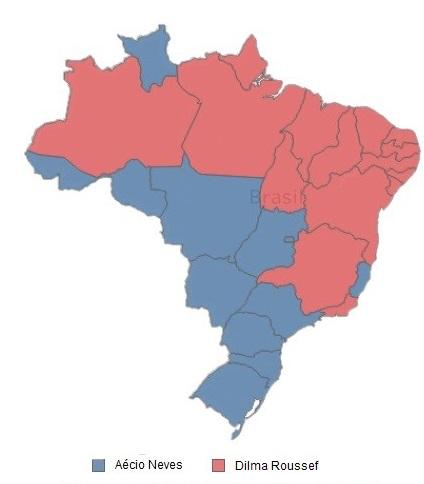
\includegraphics[height=5cm]{mapaTse} \quad
        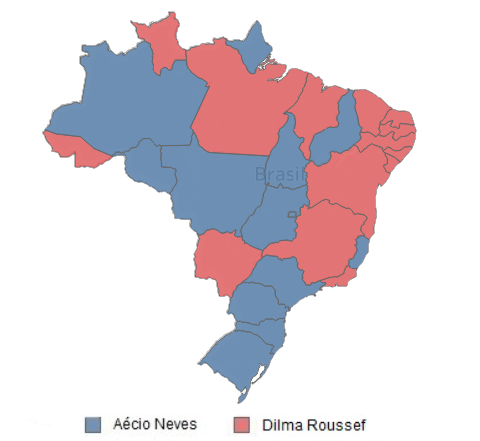
\includegraphics[height=5cm]{Prediction}
    \caption{Comparação do Resultado das eleições presidenciais de 2014 pelo \acrshort{TSE} com a predição obtida pelo \textit{framework}} \label{gdimotes}
    \label{eleicoes}
    \end{center}
    \end{figure}
    
 
 
 
 \section{Plataforma de Análise de Sentimentos \textit{Online}}
 
 Como resultado deste trabalho foi desenvolvida uma interface online para classificação automática de novos textos
 extraídos de redes sociais. Na Figura \ref{tela_principal} é detalhada a tela principal que serve para que o usuário
 envie o arquivo extraído do \textit{twitter} para análise. Foi utilizado o modelo criado de forma persistiva do algoritmo 
 \acrshort{SVM}.
 
 
 \figuraBib{tela_principal}{Tela principal do protótipo de classificação automática de textos provenientes de redes sociais}{}{tela_principal}{width=0.8\textwidth}%
 
Um novo experimento foi realizado para prever os resultados do segundo turno das eleições presidenciais de 2018 previstos pela plataforma de 
análise de sentimentos online. Durante o dia das eleições, em 28 de outubro de 2018, foram extraídos do site do TSE dados 
referentes aos candidatos Fernando Haddad e Jair Bolsonaro. Com o objetivo de agrupar um grande volume de dados para classificação,
 os tweets foram extraídos da base de dados do Twitter com periodicidade de uma hora ao longo do dia das eleições. 
 Nesse processo foram extraídos mais de 200.000 tweets por candidato, totalizando mais de 400.000 linhas de informações. 
 A Figura \ref{frame_classificador} apresenta uma tela contendo os detalhes do dataset utilizado para a análise de sentimentos,
 contendo várias informações dos tweets, tais como nome do autor, data, hora, conteúdo, geolocalização e polaridade.
 
 \figuraBib{frame_classificador}{Tela com o resultado das análises utilizando o modelo desenvolvido}{}{frame_classificador}{width=\textwidth}%
 
 A avaliação de cada sentimento no decorrer da eleição pode ser visualizada na Figura \ref{bolsonaro_haddad}, onde é possível ver a diferença 
 entre os dois candidatos no que diz respeito a polaridade positiva. Neste trabalho, consideramos palavras de cunho positivo como pessoas que votam 
 no candidato Jair Bolsonaro, enquanto que as palavras negativas são consideradas como críticas de eleitores de outros candidatos.

 \figuraBib{bolsonaro_haddad}{Evolução do sentimento referente a cada candidato ao longo do dia da votação}{}{bolsonaro_haddad}{width=0.8\textwidth}%
 
 A contabilização dessa análise pode ser vista na Tabela \ref{tb:bolso_haddad}, onde o resultado é favorável ao candidato Jair Bolsonaro, que obteve um total de 54,47% de análises positivas, contra 41,38% de Haddad.
 
 
 \begin{table}
     \label{tb:bolso_haddad}
     \centering
     \caption{Classificação dos dados utilizando o modelo construído para o segundo turno das eleições presidenciais de 2018}
    
     \begin{tabular}{llll}
     \hline
               & Positivo & Neutro & Negativo \\ \hline
     Bolsonaro  & 54.47\%  & 30.88\% & 14.63\%  \\ \hline
     Haddad     & 41.38\%  & 42.95\% & 15.66\%  \\ \hline
     \end{tabular}
 \end{table}
 
 
 Como as eleições brasileiras utilizam as urnas eletrônicas durante o processo eleitoral, é possível saber 
 quem ganhou somente após a finalização da votação no último colégio eleitoral do Brasil, que é o estado do Acre. Na Tabela
 \ref{tb:tse2018} apresenta o resultado oficial do \acrshort{TSE}.
 
 
 \begin{table}[tbp]
     \centering
     \caption{Distribuição dos resultados da eleição presidencial de 2018}
     \label{tb:tse2018}
     \begin{tabular}{ll}
     \hline
     Bolsonaro & 55,13\% \\ \hline
     Haddad & 44,87\% \\ \hline
     \end{tabular}
 \end{table}
 
 
 Ao comparar o resultado do \textit{framework} com o resultado oficial das eleições brasileiras, verifica-se que as predições do modelo obtiveram resultado satisfatório. A utilização da geolocalização nessa etapa não ofereceu bons resultados, visto que
 a \acrshort{API} do \textit{Twitter} passou por várias atualizações e limitou as requisições para 5,000 por dia, impossibilitando 
 uma análise detalhada da localização de cada \textit{tweet} postado. Outra limitação é que, por se tratar de redes sociais, as pessoas
 não têm uma obrigação legal de inserir a sua localização exata.